\documentclass[a4paper]{article}

\usepackage{inputenc}
\usepackage[british,UKenglish]{babel}
\usepackage{amsmath}
%\usepackage{titlesec}
\usepackage{color}
\usepackage{graphicx}
\usepackage{fancyref}
\usepackage{hyperref}
\usepackage{float}
\usepackage{scrextend}
\usepackage{setspace}
\usepackage{xargs}
\usepackage{multicol}
\usepackage{nameref}

\usepackage{sectsty}
\usepackage{multicol}
\usepackage{multirow}
\usepackage[procnames]{listings}
\usepackage{appendix}
\usepackage{listings}

\newcommand\tab[1][1cm]{\hspace*{#1}}
\hypersetup{colorlinks=true, linkcolor=black}
\interfootnotelinepenalty=10000

\newcommand{\cleancode}[1]{\begin{addmargin}[3em]{3em}\texttt{\textcolor{cleanOrange}{#1}}\end{addmargin}}
\newcommand{\cleanstyle}[1]{\text{\textcolor{cleanOrange}{\texttt{#1}}}}


\usepackage[colorinlistoftodos,prependcaption,textsize=footnotesize]{todonotes}
\newcommandx{\commred}[2][1=]{\textcolor{Red}
{\todo[linecolor=red,backgroundcolor=red!25,bordercolor=red,#1]{#2}}}
\newcommandx{\commblue}[2][1=]{\textcolor{Blue}
{\todo[linecolor=blue,backgroundcolor=blue!25,bordercolor=blue,#1]{#2}}}
\newcommandx{\commgreen}[2][1=]{\textcolor{OliveGreen}{\todo[linecolor=OliveGreen,backgroundcolor=OliveGreen!25,bordercolor=OliveGreen,#1]{#2}}}
\newcommandx{\commpurp}[2][1=]{\textcolor{Plum}{\todo[linecolor=Plum,backgroundcolor=Plum!25,bordercolor=Plum,#1]{#2}}}

\def\code#1{{\tt #1}}

\def\note#1{\noindent{\bf [Note: #1]}}

\makeatletter
%% The "\@seccntformat" command is an auxiliary command
%% (see pp. 26f. of 'The LaTeX Companion,' 2nd. ed.)
\def\@seccntformat#1{\@ifundefined{#1@cntformat}%
   {\csname the#1\endcsname\quad}  % default
   {\csname #1@cntformat\endcsname}% enable individual control
}
\let\oldappendix\appendix %% save current definition of \appendix
\renewcommand\appendix{%
    \oldappendix
    \newcommand{\section@cntformat}{\appendixname~\thesection\quad}
}
\makeatother




\lstset{frame=, basicstyle={\footnotesize\ttfamily}}



\graphicspath{ {images/} }
\usepackage{ctex}
%-----------------------------------------BEGIN DOC----------------------------------------

\begin{document}
\renewcommand{\contentsname}{目\ 录}
\renewcommand{\appendixname}{附录}
\renewcommand{\appendixpagename}{附录}
\renewcommand{\refname}{参考文献} 
\renewcommand{\figurename}{图}
\renewcommand{\tablename}{表}
\renewcommand{\today}{\number\year 年 \number\month 月 \number\day 日}

\title{{\Huge 考前突击指南{\large\linebreak\\}}}
%please write your name, Student #, and Class # in Authors, student ID, and class # respectively
\author{\\徐\ 国\ 栋\\
自动化\ 1402\ 班}
\date{\today}
\maketitle
\newpage

%-----------------------------------------ABSTRACT-------------------------------------
% \begin{center}
% {\Large\bf{摘\ 要\\}}
% \end{center}
% 请在这里输入摘要内容.
% \newpage
%-----------------------------------------ABSTRACT-------------------------------------
% \begin{center}
% {\Large\bf{版\ 权\ 声\ 明\\}}
% \end{center}
% 该文件受《中华人名共和国著作权法》的保护。...保留拒绝授权违法复制该文件的权利。任何收存和保管本文件各种版本的单位和个人,未经....同意,不得将本文档转借他人,亦不得随意复制、抄录、拍照或以任何方式传播。 否则,引起有碍著作权之问题,将可能承担法律责任。\newpage
%-----------------------------------------CONTENT-------------------------------------
\begin{center}
\tableofcontents\label{c}
\end{center}
\newpage

%------------------------------------------TEXT--------------------------------------------

%----------------------------------------OVERVIEW-----------------------------------------

\section{考前突击指南} \label{overview}%------------------------------
本指南主要针对考前突击,基本0基础但是想要获得高分(90-100)的同学。时间最好能有1-2周,有很多课的话其实可以并行这样学习。当然不推荐想认真学习的同学用这种方法。因为考前突击遗忘率是很高的,可能考完没几天就忘的差不多了,当然想重新捡起来也是很快的,看大家个人需求啦\ :) 。

\subsection{绩点的重要性} \label{sub:importance}
绩点很重要,不论是出国还是保研,绩点都是你申请的时候最重要的一栏。当然整个申请过程当然不是只看绩点,但是绩点相当于一张能够进入复试的门票,所以让我们重视起来~

\subsection{资料准备} \label{sub:prepare}
因为我是工科,不知道文科的情况,所以也没办法覆盖所有的情况,但是基本能覆盖大部分的课程了。前期我们需要花一点时间准备复习资料。这部分一般我会一次性把所有课程需要的资料全部准备好,主要是电子版的资料+纸质课本(辅导书)+纸质往年试w卷这三种,电子版的资料按照课程在电脑上划分好文件夹,方便查找。

\begin{itemize}
	\item{\textbf{获取往年真题以及老师布置的作业:} 这个很重要,一般一门课都会有往年积累下来的考卷,常见的来源包括:南湖打印店,百度文库,豆丁,学长学姐留下来的.....等等,这个靠大家自己搜索了。一般大一大二的课这类资源比较多,大三的专业课可能更多要在学院内找了。老师布置的作业考的几率也很大,要弄懂。}
    \item{\textbf{复习课或者老师在平时透露的可能的考点:} 这个就需要在最后一两节课认真停下老师怎么复习的了,注意划重点。还可以找听课较多的学霸,看看他们知道不知道哪部分会考,这部分可以自己总结好了打印下来看。}
    \item{\textbf{网上下一些该课程的复习材料:} 找一两个网上的就行了,不一定需要是我们学校的,但是最好是那种把课程总结的很全的材料。}
    \item{\textbf{老师指定的教材+辅导教材:} 课后习题是很大的题库来源。}
    \item{\textbf{老师的PPT:} 上面的题一般也很多,用来复习很好,有人只看这个。}
\end{itemize}

总之,按照资料的重要性排序的话。

\begin{itemize}
	\item{往年的考试真题}
    \item{老师布置的课后作业,老师发的复习资料,PPT。}
    \item{教材课后习题。}
    \item{网上的非本校的试卷。(3,4的重要程序可能要依赖课程决定)}
    \item{教材自身}
\end{itemize}

\subsection{开始复习} \label{sub:start}
有了以上5个材料,我们就可以开始一门课程的复习了,一般可以按照下面的步骤来复习一门课。
\begin{itemize}
	\item{\textbf{了解课程的思维,解题模式} 看教材的目录,了解这门课在讲什么,根据几个章节的题目及其子题目,在心中建立该学科的思维框架,模式。这部分很重要,最好在开始的时候掌握,对后面的复习有很大的指导意义,可以配合前言,绪之类的一起看。}
    \item{\textbf{逐步复习} 一天1-3章的速度把整本书过一遍,速度自行控制,如果有辅导材料一定要买(图书馆可以借,对理解很有帮助),类似形式的资料还有老师的PPT,一起看。习题要看,直接看答案就可以了,看懂即可,重要的是了解做题的思维模式。}
    \item{\textbf{总体复习} 完成2之后,看一下大纲性质的复习材料,这部分可以是网上找的,如果老师有发最好,这时候大部分的东西基本都能理解了,一门课的常见范式我们也基本了解了,如果有时间,在快速把整本书看一遍,串起知识点。}
    \item{\textbf{刷题} 完成3之后,刷老师布置的作业+往年的考试卷纸,如果没有的话,去网上找卷子刷+课后习题基本弄懂。}
\end{itemize}

刷题一个准则是\textbf{不要花太多时间自己想,直接看答案弄懂即可,要确保下次遇到这个题或者该类型的题能做出来},不然时间可能不够,当然这不一定适合所有人。

\newpage

%------------------------------------Lab Process--------------------------------------

%------------------------------


% \section{PTX指令序列产生}\label{sub:ptx}
% \subsection{实验过程} \label{sub:ptxproc}
% 建议使用listings package来表示不同显示不同的命令行或代码。使用如下代码:
% \begin{lstlisting}[language=bash]
% $source setup release
% \end{lstlisting}
% 如果使用图进行说明,Latex中插入图并进行索引的方式如下:图\ref{fig:singleblock}. 
% \begin{figure}[ht]
%  \centering
%  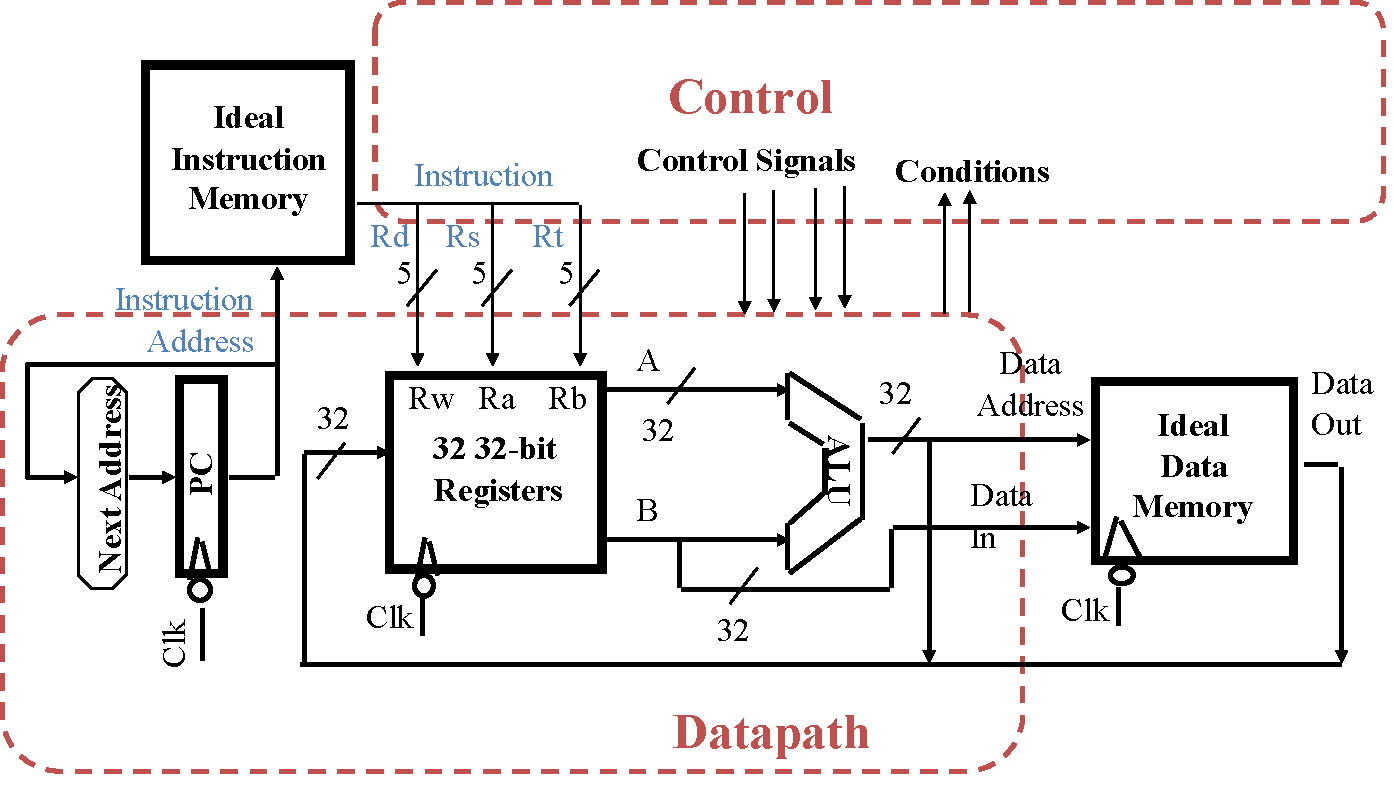
\includegraphics[height=5cm]{images/l1sys.pdf}
%  \caption{单周期处理器结构图}
%  \label{fig:singleblock}
% \end{figure}
% 如果需要索引参考文献,请使用\cite{Erdos01}, 同时已经将参考文献的项目模版在文末写出。

% 如果需要表格,可以建立类似表\ref{tab:signaldef}这样的列表进行说明。

% \begin{table}[htp]
% \caption{测试模式信号定义}\label{tab:signaldef}
% \begin{center}
% 	\begin{tabular}{|l|l|l|p{6cm}|}
% 	\hline
% 	\textbf{信号名} & \textbf{方向} & \textbf{位宽} & \textbf{功能描述}\\ \hline \hline
% 	boot			& Input 	& 1-bit	& 触发测试模式, 当处理器正常工作时被置为0\\ \hline
% 	test\_im\_wr 	& Input	& 1-bit	& Instruction memory write enable in test mode,set to 0 in 	
% 								  CPU regular process mode. In test mode, it will be set to 1 when if writing instructions to imem, otherwise it is set to 0.\\ \hline
% 	test\_im\_re 	& Input & 1-bit & Instruction memory read enable in test mode,set to 0 in 	
% 								  CPU regular process mode. In test mode, it will be set to 1 when if reading instructions out, otherwise it is set to 0. \\ \hline
% 	test\_im\_addr 	& Input & 32-bit& Instruction memory address\\ \hline
% 	test\_im\_in 	& Input & 32-bit& Instruction memory data input for test mode. \\ \hline
% 	test\_im\_out 	& Output& 32-bit& Instruction memory data output for test mode. \\ \hline
% 	test\_dm\_wr 	& Input	& 1-bit	& Data memory write enable in test mode,set to 0 in 	
% 								  CPU regular process mode. In test mode, it will be set to 1 when if writing data to dmem, otherwise it is set to 0.\\ \hline
% 	test\_dm\_re 	& Input & 1-bit & Data memory read enable in test mode,set to 0 in 	
% 								  CPU regular process mode. In test mode, it will be set to 1 when if reading data out, otherwise it is set to 0.\\ \hline
% 	test\_dm\_addr 	& Input & 32-bit& Data memory address\\ \hline
% 	test\_dm\_in 	& Input & 32-bit& Data memory input for test mode. \\ \hline
% 	test\_dm\_out 	& Output& 32-bit& Data memory output for test mode. \\ \hline
% 	valid			& Output& 1-bit & If CPU stopped or any exception happens, valid signal is set to 0.\\ 
% 	\hline
% 	\end{tabular}
% \end{center}
% \end{table}

% \subsection{实验结果和分析}\label{sub:ptxeva}
% 请在这一节详细说明需要分析的内容。
% % --------------------------------Evaluation----------------------------------------
% \section{PTX与x86指令的比较}\label{ptxvsx86}
% 以下请按照上面的说明示例,自行安排章节内容。

% % -----------------------------------Appendix----------------------------------------
% \appendix
% \section{代码}\label{sub:app.code}
% 请在附录\ref{sub:app.code}中添加代码。请使用如下C或者C++的语法高亮描述方法。
% \begin{lstlisting}[language=C]
% class TopIO extends Bundle() {
% 	val boot = Input(Bool()) 
% // imem and dmem interface for Tests
% 	val test_im_wr		= Input(Bool())
% 	val test_im_rd 		= Input(Bool())
% 	val test_im_addr 	= Input(UInt(32.W))
% 	val test_im_in 		= Input(UInt(32.W))
% 	val test_im_out 	= Output(UInt(32.W))

% 	val test_dm_wr		= Input(Bool())
% 	val test_dm_rd 		= Input(Bool())
% 	val test_dm_addr 	= Input(UInt(32.W))
% 	val test_dm_in 		= Input(UInt(32.W))
% 	val test_dm_out 	= Output(UInt(32.W))

% 	val valid			= Output(Bool())
% }
% class Top extends Module() {
% 	val io 		= IO(new TopIO())//in chisel3, io must be wrapped in IO(...) 
% 	//...
% 	when (io.boot & io.test_im_wr){
% 		imm(io.test_im_addr) := io.test_im_in
% 		} .elsewhen (io.boot & io.test_dm_wr){
% 		// please finish it
% 		} //...
% }
% \end{lstlisting}
% \newpage
% -----------------------------------REFERENCE----------------------------------------
% \begin{thebibliography}{9}
% \bibitem{Erdos01} P. Erd\H os, \emph{A selection of problems and
% results in combinatorics}, Recent trends in combinatorics (Matrahaza,
% 1995), Cambridge Univ. Press, Cambridge, 2001, pp. 1--6.
% \end{thebibliography}
\end{document}

